\chapter{Preliminary Results}\label{Ch:ResultsPrelim}

In this chapter, we briefly discuss the preliminary results we obtained on simpler games. In section \ref{sec:tabQ}, we present our successes with implementing tabular Q-learning on classic control games, Cart Pole and Mountain Car. We then show our results using deep Q-learning on a Atari game, Breakout, in section \ref{sec:deepQ}.

\section{Tabular Q-Learning Results}\label{sec:tabQ}

\begin{figure}[h!]
\centering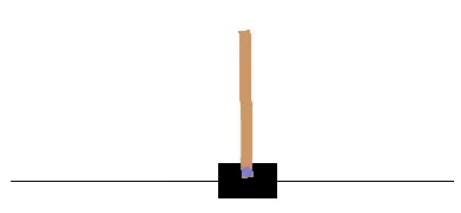
\includegraphics[scale=0.45,clip]{Graphics/cartpole.png}
\caption[Cart Pole]{The game environment of a simple classic control game, Cart Pole}
\label{fig:cartpole}
\end{figure}

We initially investigated two simple games from the OpenAI Gym toolkit. The first game was Cart Pole, where the goal is to balance a pole in a cart for as long as possible. In this game, the state is represented as a four-dimensional vector containing the values for the position of the cart, the velocity of the cart, the angle of the pole, and the velocity of the pole. The game is considered solved when the agent achieves an average score $\geq$ 195 over 100 consecutive trials. Using the tabular Q-learning approach, the algorithm achieved a perfect score of 200 over 100 consecutive trials. This score was achieved with a bucket size of 1 for the position and velocity of the cart and a bucket size of 20 for the angle and velocity of the pole for state space discretization. This agent was trained for 500 episodes with a discount factor of 0.99, minimum learning rate of 0.05, and minimum explore rate of 0.1.

\begin{figure}[h!]
\centering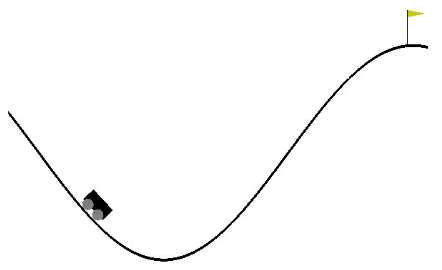
\includegraphics[scale=0.45,clip]{Graphics/mountain_car.png}
\caption[Mountain Car]{The game environment of a simple classic control game, Mountain Car}
\label{fig:mountain_car}
\end{figure}

We also trained the tabular Q-learning algorithm for the Mountain Car game. In this game, the goal is for the car to reach the top of the mountain as quickly as possible. We initially faced challenges with this game due to the nature of the reward function. Since the reward function returns a negative reward for each time step, it is difficult to reinforce positive behavior before actually winning the game. As a result, the performance varied as a result of slight changes in parameters. After experimentation, the algorithm performed best with a bucket size of 10 for position, bucket size 30 for velocity, discount factor of 0.99, fixed learning rate of 0.05 and fixed explore rate of 0.1. After training for 10,000 episodes, the algorithm achieved an average reward of -157.64 over 100 test episodes.

\section{Deep Q-Learning Results}\label{sec:deepQ}
Next, we implemented the Deep Q-Learning algorithm on the Atari Breakout and Pong games using the convolutional architecture as defined in \cite{mnih2013playing}. The first layer of the neural network was a convolutional layer with 32 kernels, 8x8 filter, and stride 4x4. The second was a convolutional layer with 16 kernels, 4x4 filter, and stride 2x2. The third layer was a dense layer with 256 neurons and a nonlinear rectifier. The final layer was a dense layer with 16 neurons and a linear rectifier. The performance was quantitatively analyzed using average Q-values. Assuming that $S$ is a uniform sample of $n$ fixed states, an estimate of the average Q-value was computed as follows.
$$ Q_{avg} = \frac{1}{n} \sum_{i=1}^{n} max_{a} Q(s_{i},a) ~~~ s_{i} \in S$$

Using this architecture, the algorithm was able to achieve promising results on both Breakout and Atari with the former shown in \ref{fig:breakout}. The average Q-value appeared to increase over time and eventually converge, essentially recreating the results described in \cite{mnih2013playing}.

\begin{figure}[h!]
\centering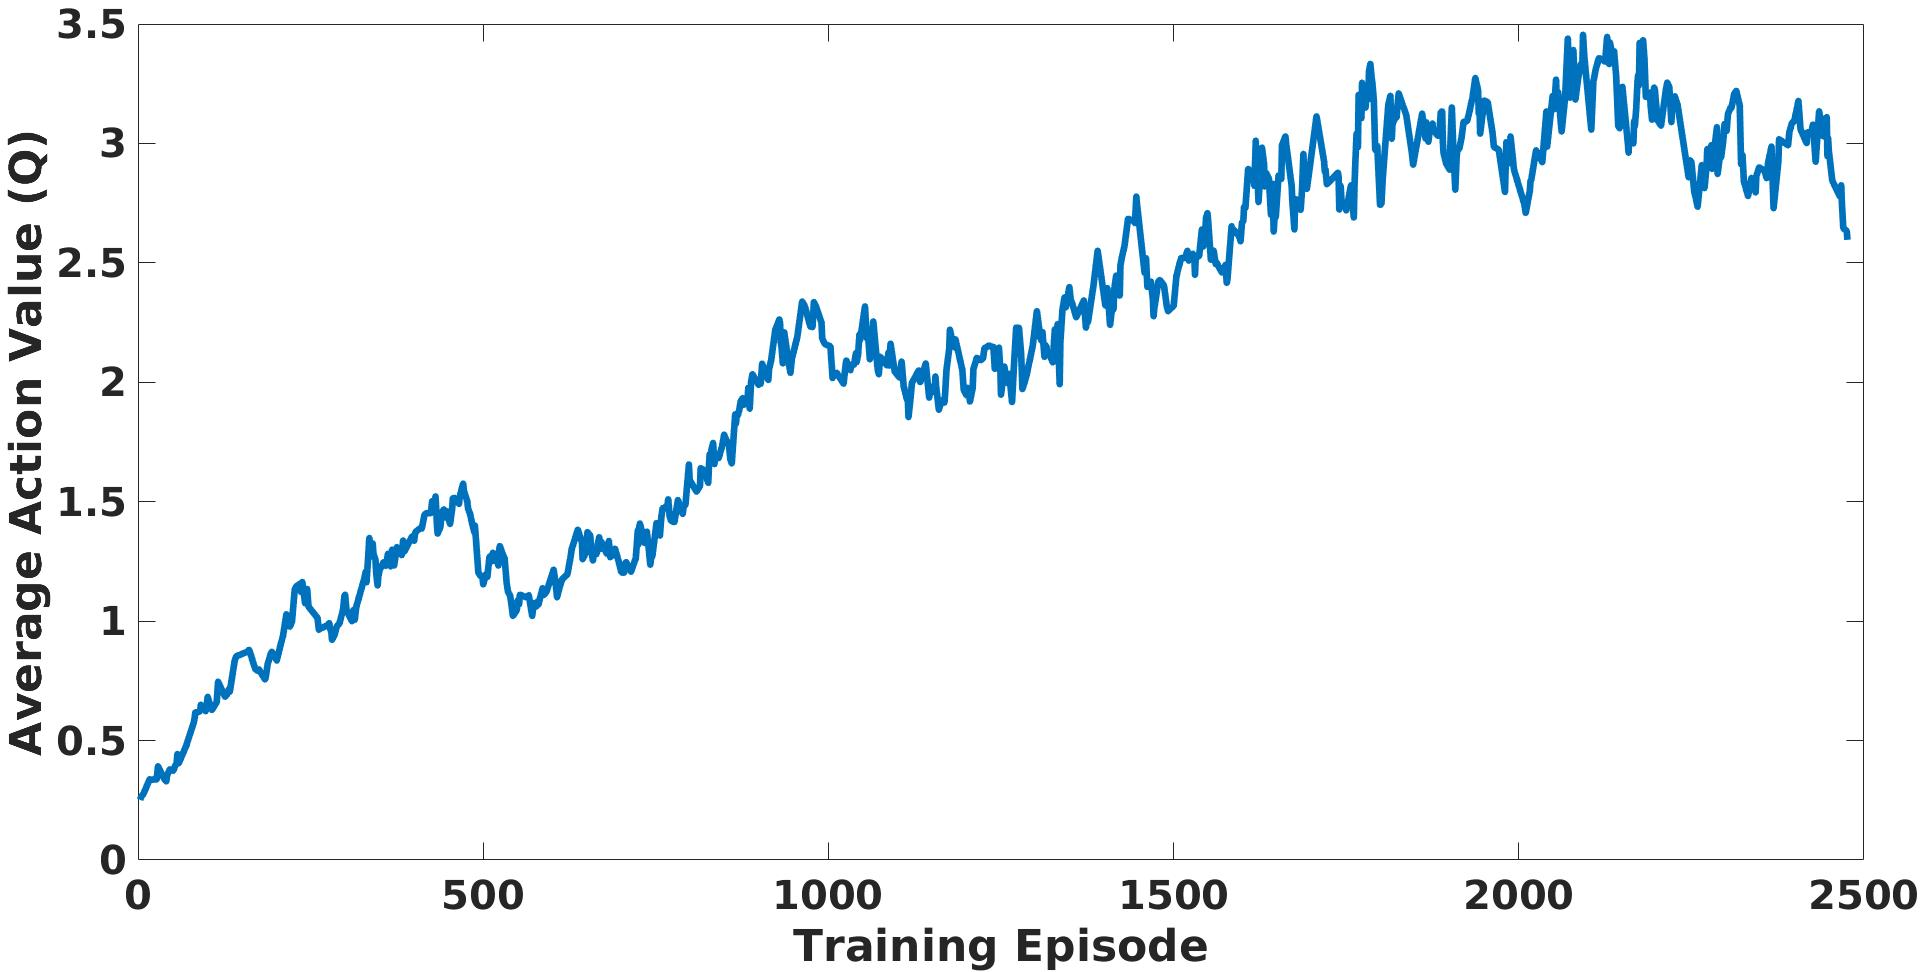
\includegraphics[width=0.6\textwidth]{Graphics/breakout_AveQ.jpg}
\caption[Average Action Value Plot for Breakout]{Average action value converges as expected}
\label{fig:breakout}
\end{figure}

\endinput



